\documentclass[a4paper,12pt]{report}

\usepackage{alltt, fancyvrb, url}
\usepackage{graphicx}
\usepackage[utf8]{inputenc}
\usepackage{hyperref}
\usepackage{setspace}
\usepackage{wrapfig}
\usepackage{xcolor}

% Questo commentalo se vuoi scrivere in inglese.
\usepackage[italian]{babel}

\usepackage[italian]{cleveref}

\title{Relazione\break``IOT Assignment 3''}

\author{Linda Fabbri, \\ Federico Raffoni,\\ Simone Rega}
\date{22 Luglio 2022}


\begin{document}
	\maketitle
	\tableofcontents
	
	\chapter{Descrizione del Sistema}
		Il progetto si pone come obiettivo quello di creare uno Smart Garden.
		Per la realizzazione di esso ci siamo basati sulle direttive e sui requisiti forniti dal prof.
	\begin{itemize}
		\item 	un ESP32 \textit{(SensorBoard)} che manda i dati delle letture dei sensori tramite richieste HTTP al server;
		\item  un server in python \textit{(Service)} che gestisce tutte le richieste HTTP e in Seriale , il quale dopo aver letto tutti i dati ed averli elaborati, spedisce all'arduino un JSON contente i dati necessari per poter azionare i led e il motore;
		\item un arduino \textit{(Controller)} che è stato implementato con una FSM, si è deciso si suddividere le operazioni principali in 3 task che vengono periodicamente chiamate da uno scheduler, l'arduino si occupa esclusivamente di  fare ciò che il server gli dice, l'unica eccezione è per quanto riguarda la comunicazione Bluetooth, in quanto essendo un canale Seriale diretto tra App e Arduino, quest'ultimo si preoccuperà di fornire i dati al server .
		\item 	un \textit{App Mobile} implementata in Java tramite Android Studio, ha una grafica simile all'esempio mostrato nelle direttive ed ha un implementazione minimale, con l'unico scopo di fornire dati real-time all'arduino
		\item una pagina web \textit{(Dashboard)} da cui poter vedere le informazioni principali dell'intero sistema, quindi il suo stato, lo stato delle luci, dell'irrigatore ed infine anche temperatura e luminosità.
	\end{itemize}


	\chapter{Breve Descrizione FSM utilizzata}
	Abbiamo deciso di implementare l'intero sistema come una Macchina a Stati Finiti \textit{(FSM)}. Da come si poteva dedurre dalle specifiche gli stati sono 3: \textbf{AUTO}, \textbf{MANUAL}, \textbf{ALARM}.
	\begin{itemize}
		\item \textbf{AUTO}: quando siamo in modalità AUTO il server decide tutto quello che bisogna fare in base alle letture dell'esp, mandando informazioni specifiche all'arduino di cosa deve azionare o accendere. Quando è in questa modalità arduino rimane in ascolto sulla Seriale Bluetooth nel caso l'utente richiedesse l'accesso manuale al sistema. In questa modalità si può entrare in ALARM se ci sono le giuste condizioni.
		\item \textbf{MANUAL}: in questa modalità il server non manda nessun dato e si limita a leggere cosa fa arduino, l'intero sistema viene gestito dall'utente che usa l'app mobile. In questa modalità non si può entrare in ALARM.
		\item \textbf{ALARM}: quando si entra in questa modalità l'intero sistema si blocca aspettando l'intervento di un utente che sblocchi tutto dall'app mobile, dopo lo sblocco si torna in modalità AUTO
	\end{itemize}
	\chapter{Breadboard Schema}
		\begin{figure}[!htb]
			\centerline{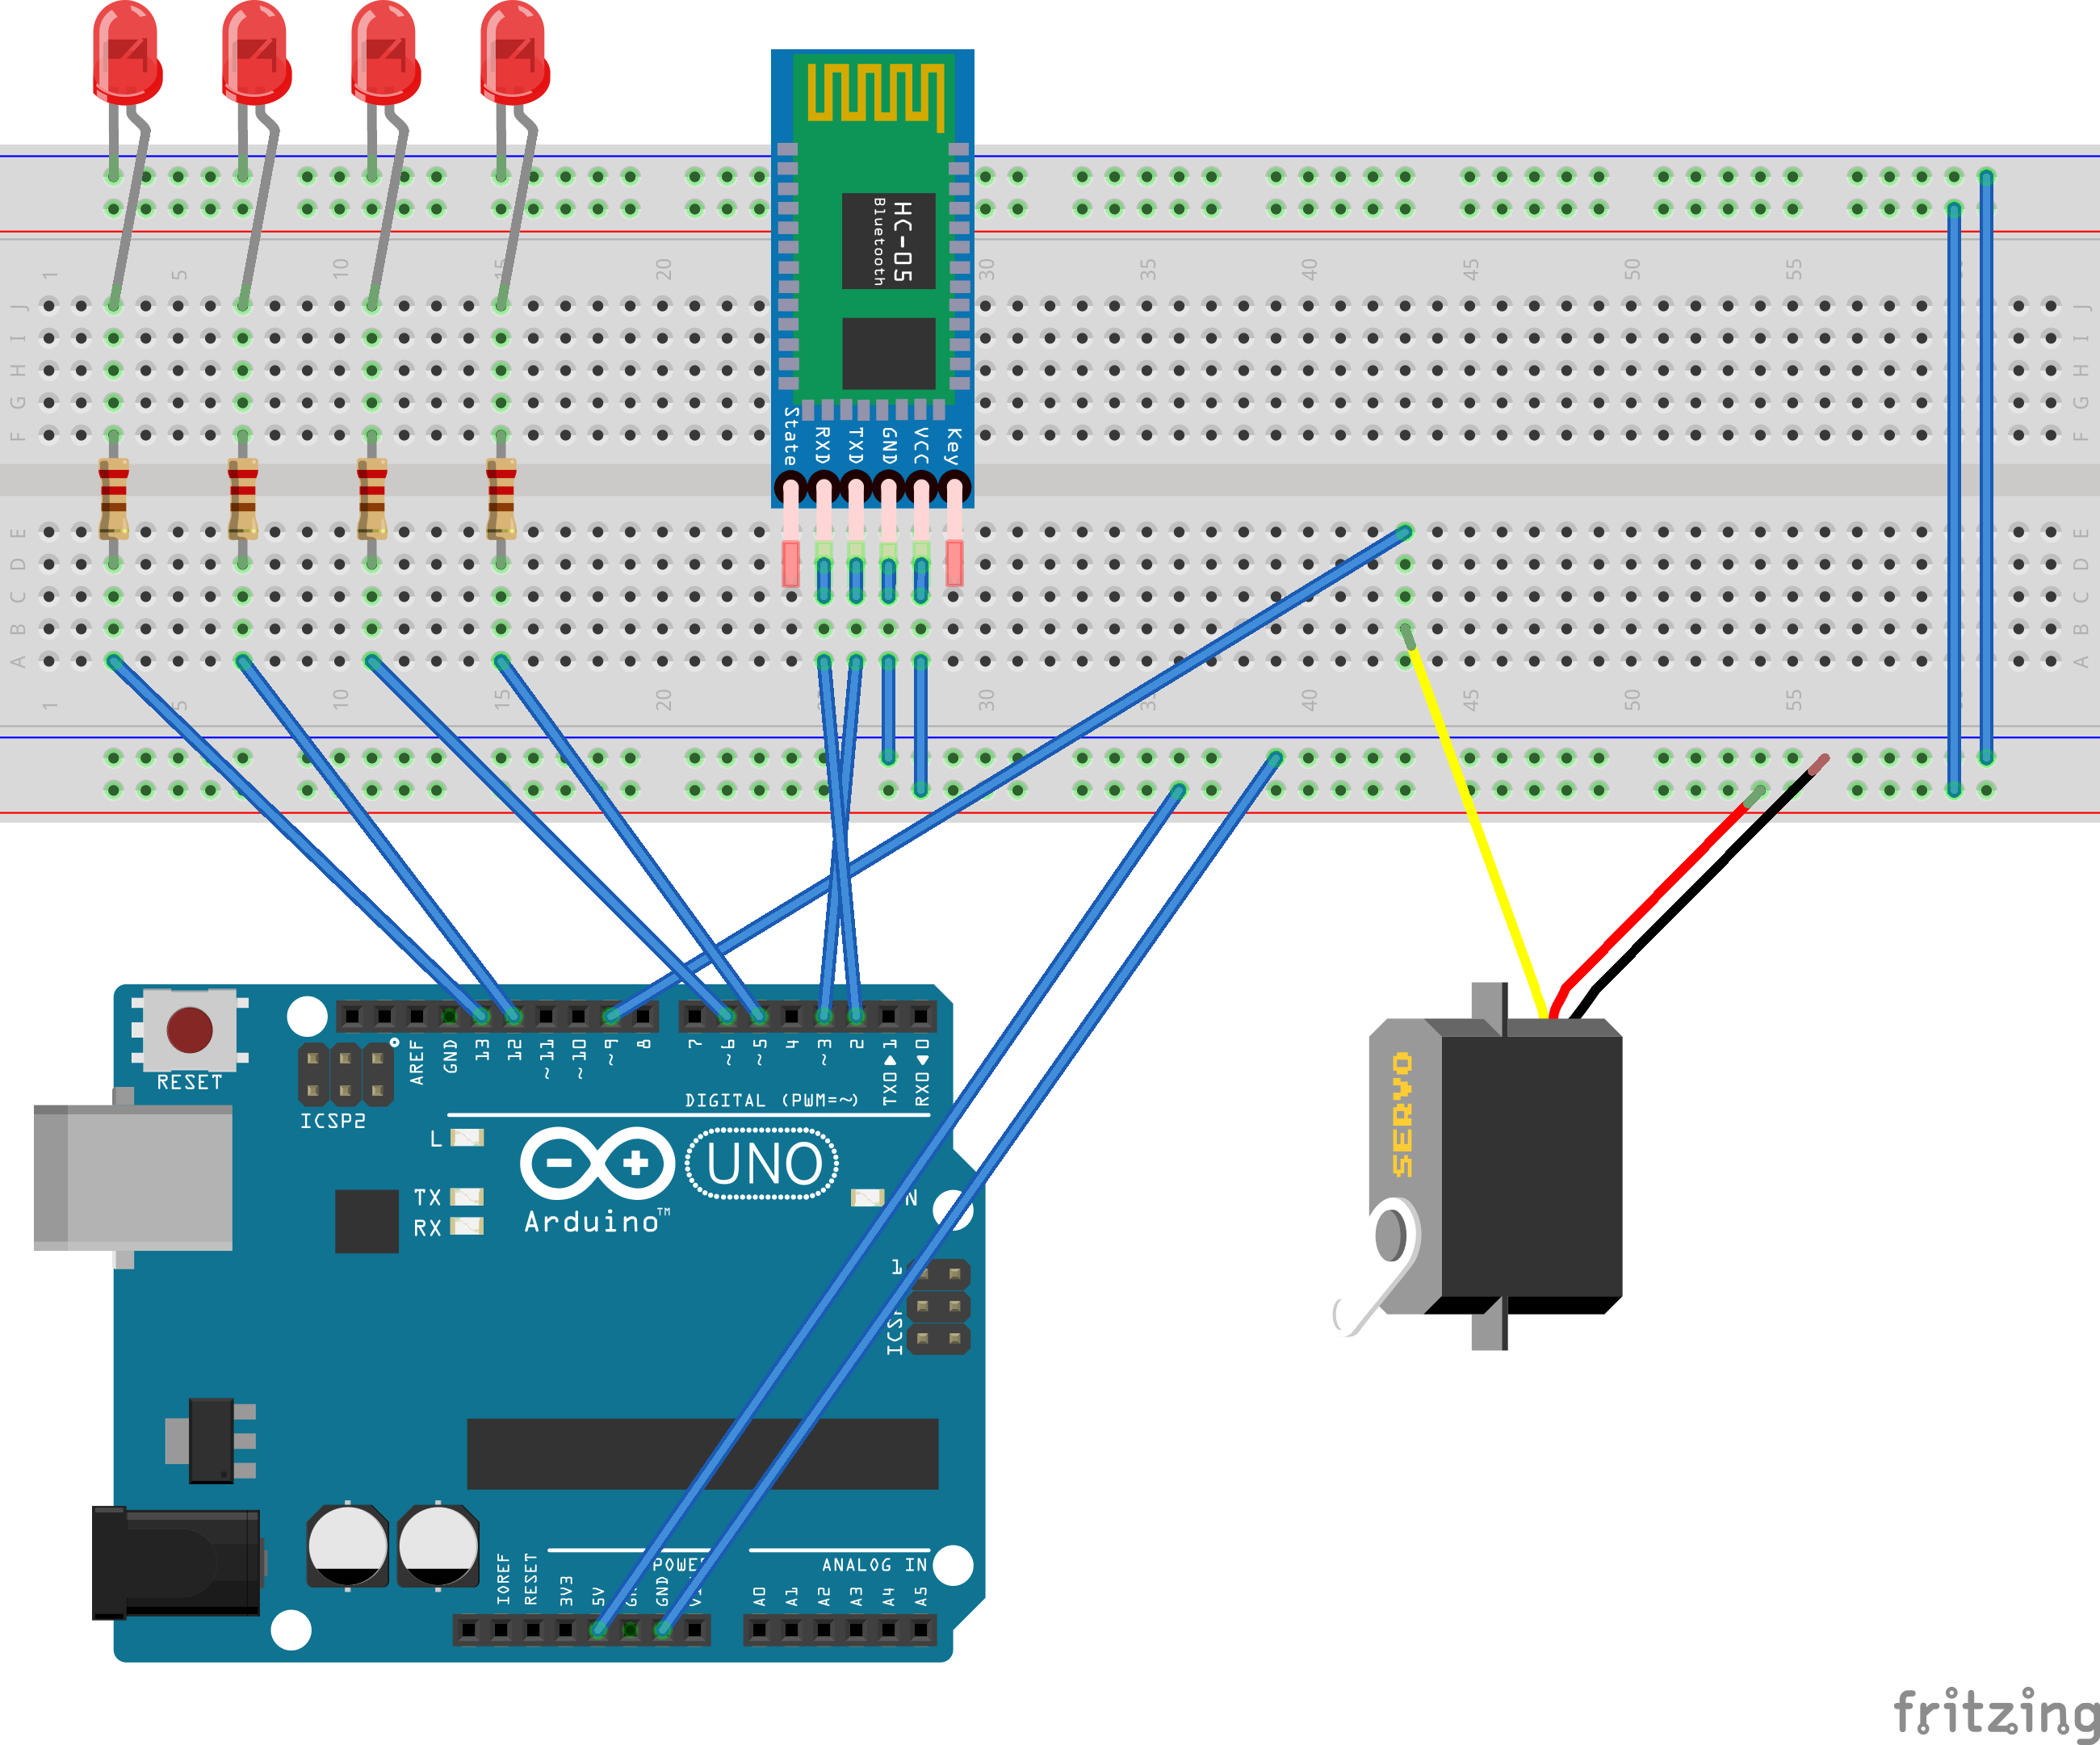
\includegraphics[scale=0.9]{iot3_bb.png}}
			\caption{Schema collegamenti di arduino e dei componenti}
			\label{img:analysis}
		\end{figure}	
	\chapter{Video}
	
	
\end{document}
